\section{Justificaci\'on del Proyecto}\label{sec:justificacion}

A medida que crece el requerimiento de ancho de banda de los usuarios
en internet, las empresas proveedoras del servicio deben utilizar más
y mejores tecnologías extensibles y flexibles que posibiliten este
proceso.

Como muestra la figura \ref{fig:aumento_bw}, el crecimiento de ancho
de banda a nivel global está en aumento constante. Se espera que este
crecimiento no se detenga nunca, ya que a medida que el ser humano
tiene acceso a más velocidad, sus necesidades y exigencias tecnológicas
aumentan.

\begin{figure}[H]
  \centering
  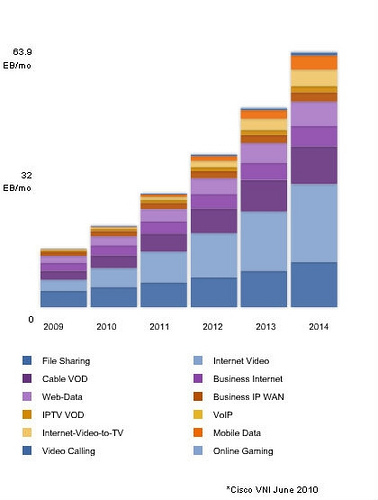
\includegraphics[width=10cm]{Imagenes/aumento_bw.png}
  \caption{Tendencia en el aumento del ancho de banda a nivel mundial
    según un estudio de Cisco de 2013.}
  \label{fig:aumento_bw}
\end{figure}

\emph{DWDM} es una tecnología en esencia modular y escalable. Todos
los proveedores de esta tecnología ofrecen actualizaciones en forma de
módulos para poder reemplazar los equipos obsoletos con versiones
nuevas o bien para expandir y mejorar el soporte de las tecnologías
tradicionales a más tendidos.

La incursión de los \emph{OADM} hacia un sistema programable con
variedad de filtros integrados y con manejo de eventos, como lo es
\emph{WSS}, ha significado que la flexibilidad de \emph{DWDM} es mayor
que nunca. Por otro lado, los precios de estos dispositivos han
disminuido de forma considerable en los últimos años, haciéndose
populares y soportados globalmente.

Las redes fotónicas ``oscuras'', es decir, sin ningún tipo de
multiplexación o control de las señales al momento de introducirlas en
la fibra, no son adecuadas para montar redes modernas que requieran
grandes anchos de banda. Este es el caso de los enlaces entre 
datacenters, donde el volumen y la importancia de los datos que fluyen
hacia y desde sus nodos deben cumplir con un tiempo de acceso cada vez
más rápido y por un número creciente de usuarios.

En efecto, lo correcto para notar esta diferencia sustancial en este
contexto es considerar la capacidad de un cable de fibra óptica con y
sin multiplexación en frecuencia. Si cada cable de G.652.D tiene 96
fibras en su interior, entonces se pueden conectar un total de 96
servicios por cada cable. Si se considera un canal de ancho 50 GHz y
protocolos Ethernet de 100 GB/s, algo totalmente admisible en una red,
la capacidad total de una fibra oscura es de 9.6 TB/s. Considerando la
misma configuración de protocolos en una red \emph{DWDM}, el cable
óptico permite el transporte de 80 veces este valor, es decir, cerca
de 768 TB/s, lo que representa una disminución de costo considerable
en términos de reparación del tendido, amplificadores y mano de obra.

Algunos de los servicios más pintorescos que permiten implementar los
data centers en el mundo son los que se muestran en la figura
\ref{fig:servicios}.

\begin{figure}[H]
  \centering
  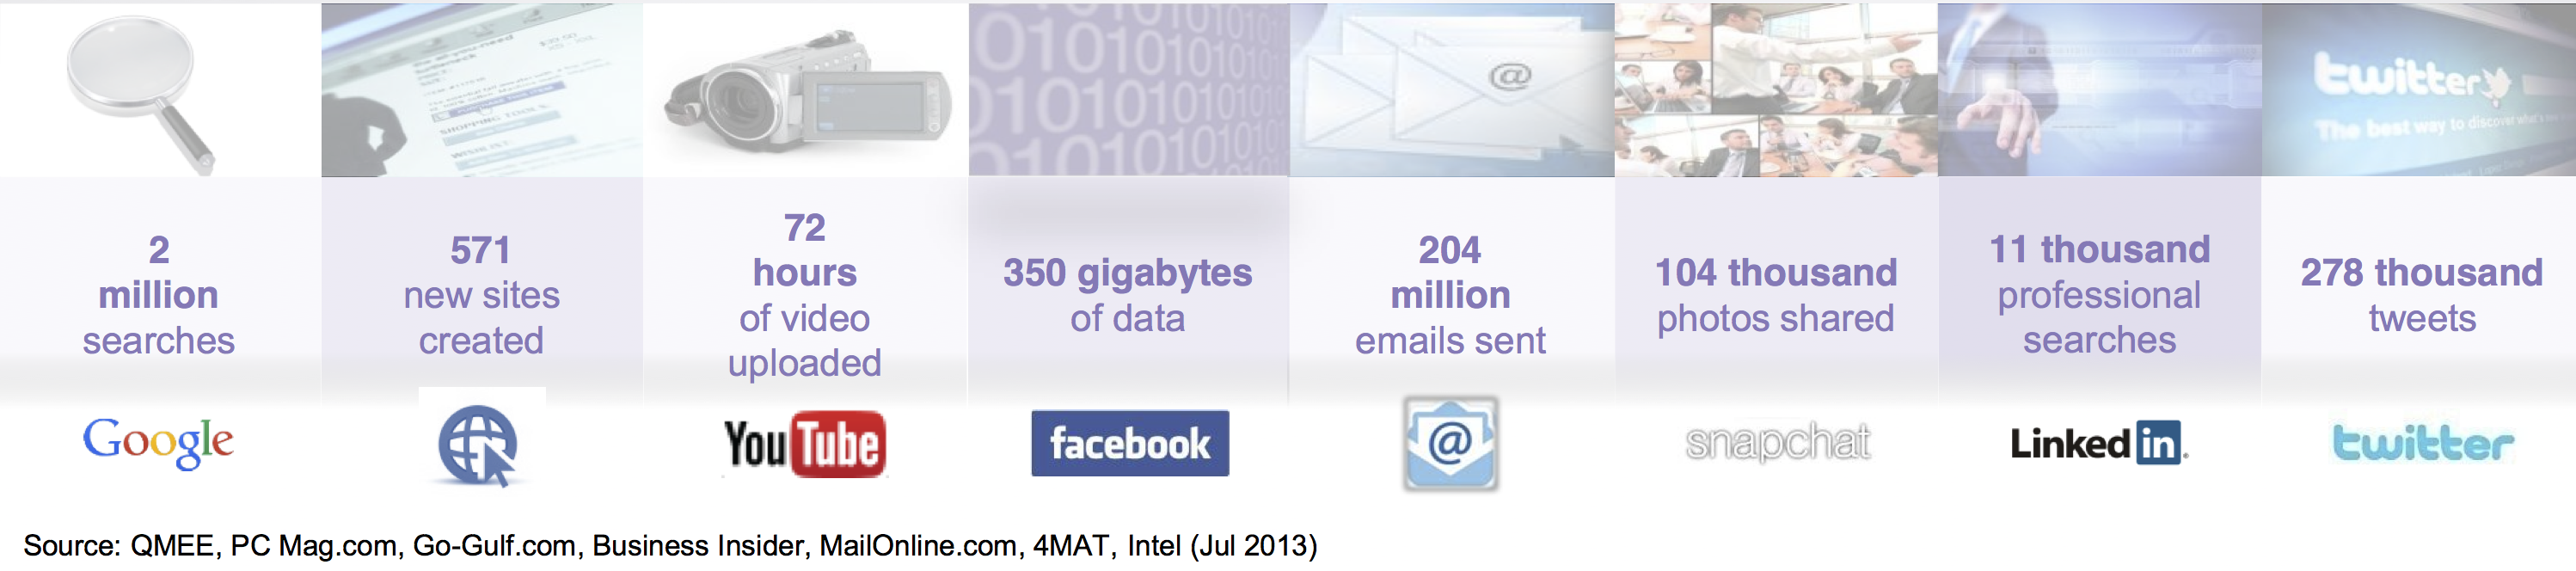
\includegraphics[width=11cm]{Imagenes/servicios.png}
  \caption{Servicios en los que participan data centers que ocupan una
    muy alta y creciente cantidad de capacidad instalada en las
    redes. Datos de julio de 2013 provenientes de: QMEE, PC Mag.com,
    Go-Gulf.com, Business Insider, MailOnline.com, 4MAT e Intel.}
  \label{fig:servicios}
\end{figure}

En definitiva, los avances, la estandarización y la disminución de 
precios que han experimentado este tipo de tecnologías son los factores 
más importantes que permiten justificar el proyecto. 
